\section{Case Studies and Evaluation}
\label{sec:experiments}

We evaluate \system on three problems selected to exercise different combinations of evidence, structural intervention, and computational validation.  The first begins with explicit two-dimensional database structures and asks the system to generate new structures after source-native bands establish the starting regime.  The second begins with a compound physical objective and requires a route-diverse portfolio.  The third is an open structural and electronic problem for which database, literature, and direct-generation routes must be combined.  All counts and numerical results below are reconstructed from archived run artifacts.

\subsection{Case study I: two-dimensional transition-metal flat bands}
\label{sec:case-flatband}

\paragraph{Goal.}
The research specification requested two-dimensional structures containing a periodic connected transition-metal sublattice, a band width no greater than 50\,meV near the Fermi level, no competing first-order or dispersive crossing at $E_\mathrm{F}$, transition-metal or transition-metal--ligand orbital character, and chemically common formal valences.  The initial C2DB search produced three explicit parents: LiP$_2$PdS$_6$, GaP$_2$PdS$_6$, and P$_2$Pd$_3$S$_8$.  Source-native PBE bands gave near-Fermi bandwidths of 267.74, 369.10, and 579.83\,meV, respectively.

The value of the run is that these parent observations became inputs to a new structural cycle.  The reasoner proposed operations against content-hashed parents, and the compiler generated four child CIFs: removal of the Li equivalent-site class from LiP$_2$PdS$_6$; two distinct Pd-equivalent-class substitutions by Ni in P$_2$Pd$_3$S$_8$; and a Pd-to-Ni substitution in GaP$_2$PdS$_6$.  The first three children retained a two-dimensional geometry, a periodic void gap of approximately 29.75--29.76\,\AA, a connected transition-metal graph, and common Pd(II)/Ni(II) assignments under the structural chemistry screen.  The fourth defined a scientifically interpretable revision route because the direct substitution led to a Ni(I) formal-valence assignment; the next proposal coupled the transition-metal change to charge compensation.

\begin{figure}[H]
    \centering
    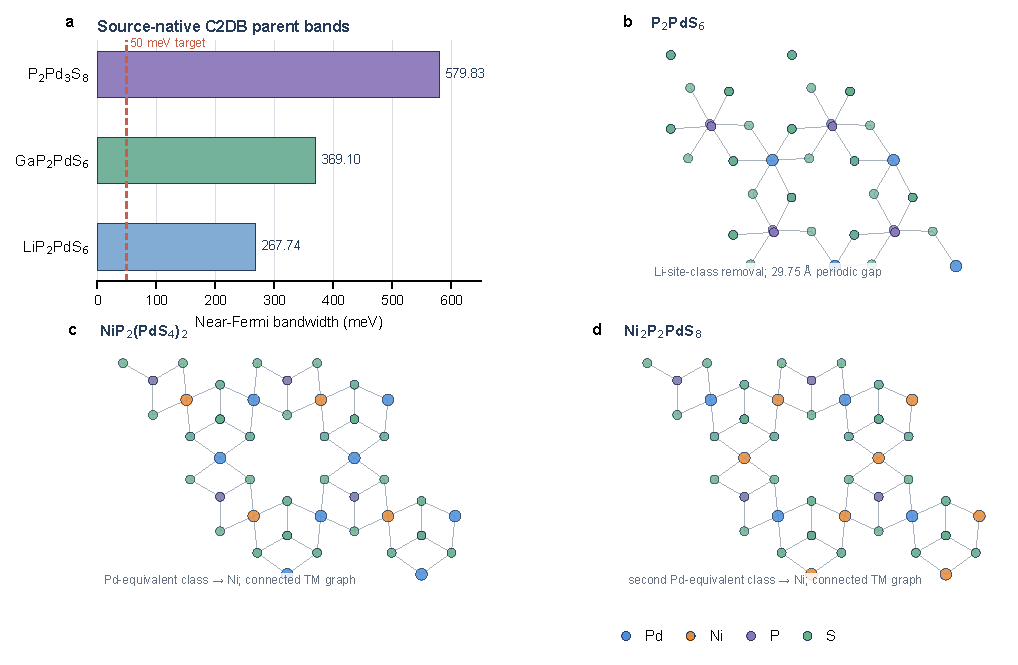
\includegraphics[width=\linewidth]{figures/prompt1-real-structures-v2.pdf}
    \caption{\textbf{Database evidence followed by explicit structure generation in the two-dimensional flat-band study.}
    (a) Source-native C2DB bands establish the bandwidth scale of the three parent structures.  (b--d) Top-view projections rendered from the generated CIF artifacts for the three children admitted by the structural hard gates.  The structures, values, and lineages are taken from the archived run; the plotting layout is generated separately for this report.}
    \label{fig:prompt1}
\end{figure}

\begin{table}[t]
    \centering
    \caption{\textbf{Structure-backed hypotheses generated in case study I.}}
    \label{tab:prompt1-children}
    \small
    \setlength{\tabcolsep}{4pt}
    \renewcommand{\arraystretch}{1.13}
    \begin{tabularx}{\linewidth}{>{\raggedright\arraybackslash}p{0.19\linewidth}>{\raggedright\arraybackslash}p{0.18\linewidth}XX}
        \toprule
        \textbf{Parent} & \textbf{Child} & \textbf{Compiled operation} & \textbf{Structure-level outcome} \\
        \midrule
        LiP$_2$PdS$_6$ & P$_2$PdS$_6$ & Remove complete Li site class & 2D, connected Pd graph, common Pd(II) \\
        P$_2$Pd$_3$S$_8$ & NiP$_2$(PdS$_4$)$_2$ & First Pd class $\rightarrow$ Ni & 2D, connected Ni/Pd graph, common Ni(II)/Pd(II) \\
        P$_2$Pd$_3$S$_8$ & Ni$_2$P$_2$PdS$_8$ & Second Pd class $\rightarrow$ Ni & 2D, connected Ni/Pd graph, common Ni(II)/Pd(II) \\
        GaP$_2$PdS$_6$ & GaNi(PS$_3$)$_2$ & Pd class $\rightarrow$ Ni & Structure retained as a charge-compensation revision route \\
        \bottomrule
    \end{tabularx}
\end{table}

This study exercises the full transition from retrieved electronic evidence to new structure records.  It also demonstrates the distinction between stages: passing the structure gates promotes a child into an electronic-screening portfolio, while the 50\,meV and orbital-character constraints remain attached as model targets.  The final products are therefore three explicit, reproducible structures and one revised chemical route, rather than a list of text-only substitutions.

\subsection{Case study II: van der Waals ferromagnetic topological materials}
\label{sec:case-vdw}

\paragraph{Goal.}
The second case asks for layered materials that combine ferromagnetism with a non-trivial spin--orbit-coupled insulating state.  \matspec decomposed the request into magnetic ground-state energy, ordering scale, SOC gap, Fermi-level placement, and a topological invariant.  Rather than reduce the search to a single chemical family, \matevidence and \mattransform organized six routes that act on different physical levers established by two-dimensional magnets and magnetic topological materials \cite{gong2017cgt,huang2017cri3,otrokov2019mnbi2te4,rienks2019hetero}.

\begin{figure}[H]
    \centering
    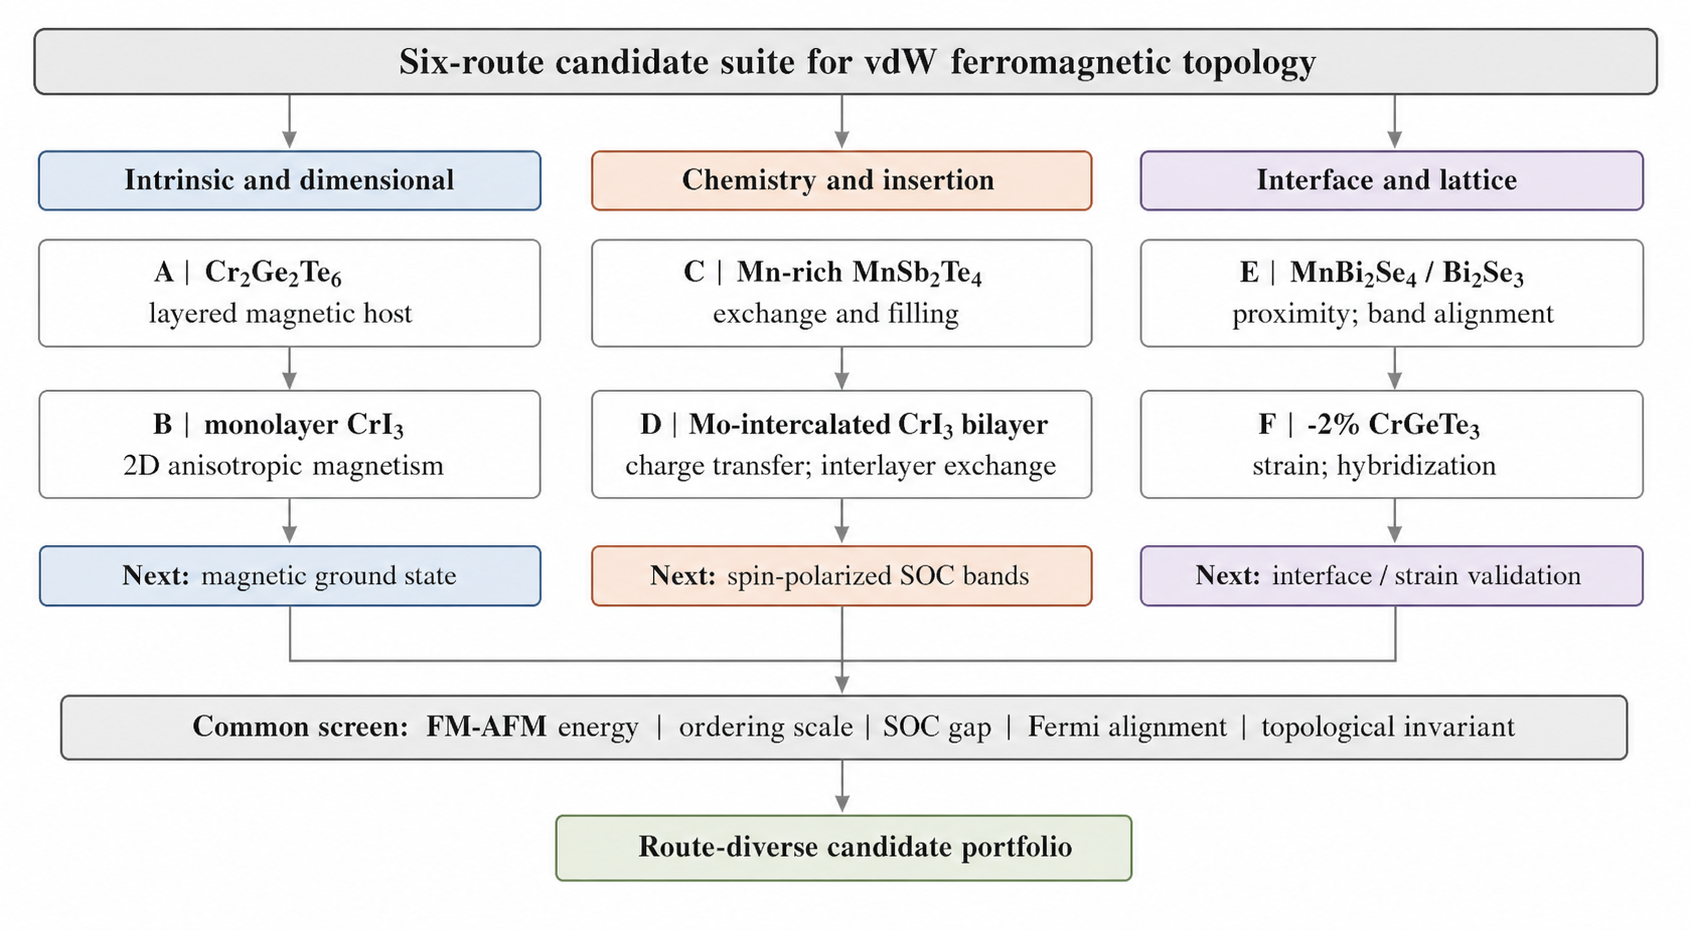
\includegraphics[width=0.88\linewidth]{figures/vdw-six-routes-image2-v3.png}
    \caption{\textbf{Six-route exploration of van der Waals ferromagnetic topology.}
    The portfolio spans intrinsic magnetic hosts, the monolayer limit, magnetic stoichiometry, intercalation, proximity coupling, and strain.  Every route is evaluated against the same five-observable verification matrix, allowing chemically distinct candidates to remain comparable.  The experiment-suite layout follows the compact evidence-column grammar used in AutoSci; the Image2-generated conceptual summary contains candidate identities and route definitions taken from the archived campaign.}
    \label{fig:vdw-routes}
\end{figure}

The intrinsic-host route retained Cr$_2$Ge$_2$Te$_6$ as a layered magnetic starting point.  The monolayer route used CrI$_3$ to focus on the dimensional dependence of ferromagnetism.  A Mn-rich MnSb$_2$Te$_4$ route varied magnetic stoichiometry in a tetradymite-related setting.  A Mo-intercalated CrI$_3$ bilayer instantiated charge-transfer and interlayer-exchange control as an intercalation plan.  A MnBi$_2$Se$_4$/Bi$_2$Se$_3$ route represented magnetic proximity and band-alignment control at a van der Waals interface.  Finally, a $-2\%$ CrGeTe$_3$ route encoded homogeneous strain as a direct structural operation.

\begin{table}[t]
    \centering
    \caption{\textbf{Route portfolio for case study II.}}
    \label{tab:vdw-routes}
    \small
    \setlength{\tabcolsep}{3.5pt}
    \renewcommand{\arraystretch}{1.12}
    \begin{tabularx}{\linewidth}{>{\raggedright\arraybackslash}p{0.20\linewidth}>{\raggedright\arraybackslash}p{0.22\linewidth}XX}
        \toprule
        \textbf{Route} & \textbf{Candidate realization} & \textbf{Primary physical lever} & \textbf{Decisive next calculation} \\
        \midrule
        Intrinsic host & Cr$_2$Ge$_2$Te$_6$ & Native layered magnetism and heavy-ligand SOC & Magnetic order plus SOC topology in the same state \\
        Monolayer limit & CrI$_3$ monolayer & Dimensionality and anisotropy & Magnetic ground state, gap and Fermi placement \\
        Stoichiometry & Mn-rich MnSb$_2$Te$_4$ & Exchange and filling through magnetic content & Competing magnetic configurations and invariant \\
        Intercalation & Mo--CrI$_3$ bilayer & Charge transfer and interlayer exchange & Relaxed registry followed by spin-polarized SOC bands \\
        Proximity & MnBi$_2$Se$_4$/Bi$_2$Se$_3$ & Exchange transfer across a vdW interface & Interface band alignment and topological invariant \\
        Strain & $-2\%$ CrGeTe$_3$ & Band inversion, hybridization and anisotropy & Strain-resolved FM--AFM energy and SOC gap \\
        \bottomrule
    \end{tabularx}
\end{table}

The route map is the principal result of this campaign stage.  Each candidate carries a different mechanism, but all share the same evidence schema and verification targets.  This makes it possible to allocate subsequent calculations by information gain: magnetic-energy calculations for routes with unresolved order, SOC calculations for candidates with an established magnetic state, and interface relaxation before electronic claims for proximity and heterostructure routes.  The system thus preserves scientific diversity without losing a common definition of success.

\subsection{Case study III: fractional-valence transition metals on a Lieb lattice}
\label{sec:case-lieb}

\paragraph{Goal.}
The third case poses an open problem: identify a crystalline material in which fractionally valent transition metals form a Lieb lattice and contribute a flat band at the Fermi level.  The compiled target requires (i) an explicit structure, (ii) non-integer average transition-metal valence compatible with charge balance, (iii) periodic Lieb connectivity of the contributing sites, (iv) a near-Fermi band width no greater than 50\,meV, (v) no disqualifying dispersive or first-order crossing, and (vi) transition-metal or hybridized ligand orbital weight.  The target connects crystalline flat-band classification, crystal-net catalogues, and electronic Lieb-lattice realizations \cite{calugaru2022flatbands,neves2024crystalnets,drost2017lieb}; no single source exposes the complete conjunction.

The campaign therefore ran three complementary routes.  The federated-database route returned 24 structures and developed seven candidate hypotheses, including cuprate, nickelate, and Pt--P/oxide-derived families.  The literature-and-mechanism route resolved 103 evidence records around six hypotheses, with layered oxyhalides such as NbOCl$_2$ and TaOCl$_2$, Ba$_2$CuO$_{3+\delta}$-related systems, and metal--inorganic-framework Lieb nets as mechanism anchors.  The structure-generation route began from three explicit database parents and produced eight intervention hypotheses, including alkali intercalation, halogen vacancy control, electrostatic gating, tensile strain, and framework routes.

The three routes were merged by candidate identity and structural lineage before model routing.  Across the consolidated campaign, 21 hypotheses yielded 17 unique structures with complete learned-Hamiltonian and band executions.  Seven operator executions produced six unique registry-child CIFs.  Four literature hypotheses without resolved structures remained linked to their mechanisms and structure-acquisition targets rather than being sent to a model with no input.

\begin{table}[t]
    \centering
    \caption{\textbf{Three-route coverage in the Lieb-lattice study.}}
    \label{tab:lieb-routes}
    \small
    \setlength{\tabcolsep}{4pt}
    \renewcommand{\arraystretch}{1.13}
    \begin{tabularx}{\linewidth}{>{\raggedright\arraybackslash}p{0.19\linewidth}c c X}
        \toprule
        \textbf{Route} & \textbf{Database leads} & \textbf{Hypotheses} & \textbf{Distinct contribution} \\
        \midrule
        Federated database & 24 & 7 & Broad structure-backed candidate discovery across four databases \\
        Literature route & 24 & 6 & Oxyhalide, cuprate and framework mechanisms linked to persistent papers and structures \\
        Structure generation & 3 & 8 & Intercalation, vacancy, gate, strain and framework interventions \\
        \midrule
        Consolidated ML campaign & \multicolumn{2}{c}{17 unique structures executed} & SOC learned-Hamiltonian bands and common hard diagnostics \\
        \bottomrule
    \end{tabularx}
\end{table}

The learned-Hamiltonian screen measured the narrowest near-Fermi band for each structure under a common 50\,meV policy.  The current closest structures were three Li$_2$Ni$_5$OF$_{11}$ vacancy-derived children with bandwidths of 60.134, 63.576, and 147.073\,meV, an NbCl$_2$O structure at 64.648\,meV, and TaCl$_2$O at 88.852\,meV.  These values re-prioritize the candidate set toward the Li--Ni oxyfluoride and oxyhalide branches.  The same band diagnostics also identify competing crossings, which become the target of the next structure and filling modifications.

\begin{figure}[H]
    \centering
    \begin{subfigure}[t]{0.48\linewidth}
        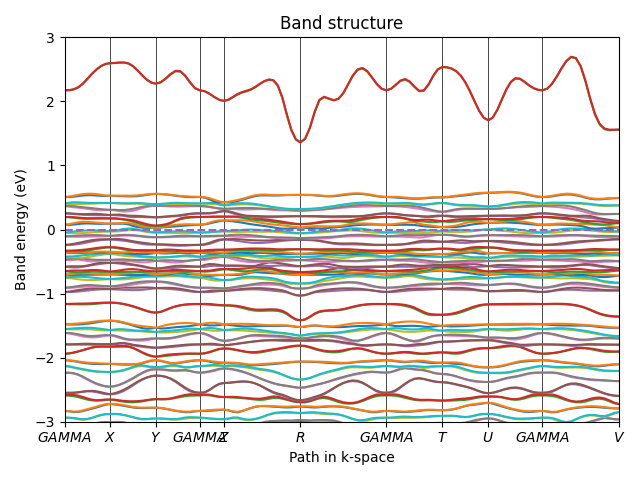
\includegraphics[width=\linewidth]{figures/lieb-li2ni5of11-band.png}
        \caption{Li$_2$Ni$_5$OF$_{11}$ child, $W=60.134$\,meV.}
    \end{subfigure}\hfill
    \begin{subfigure}[t]{0.48\linewidth}
        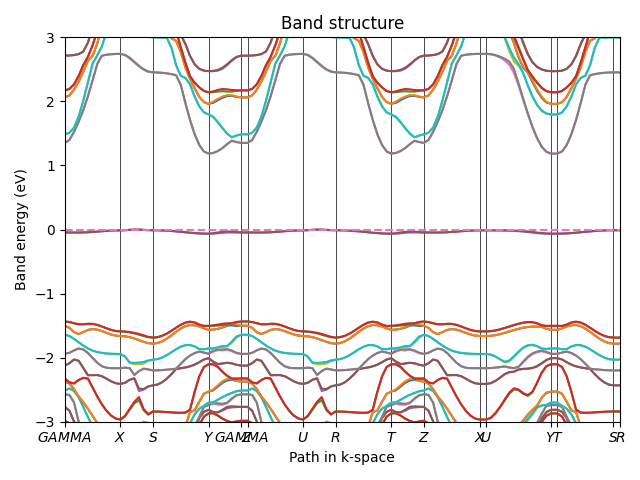
\includegraphics[width=\linewidth]{figures/lieb-nbcl2o-band.png}
        \caption{NbCl$_2$O, $W=64.648$\,meV.}
    \end{subfigure}

    \begin{subfigure}[t]{0.48\linewidth}
        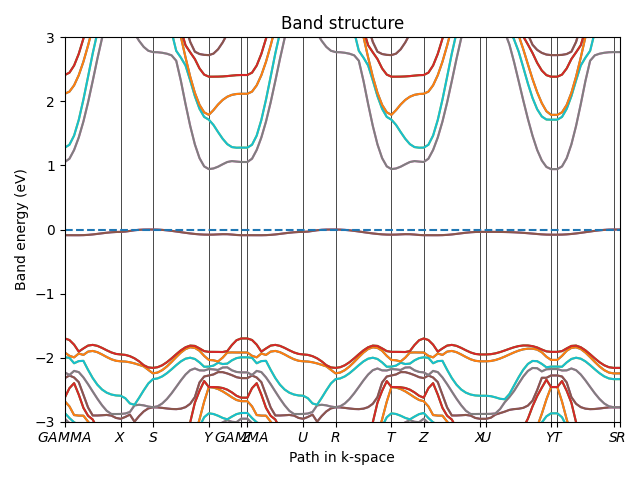
\includegraphics[width=\linewidth]{figures/lieb-tacl2o-band.png}
        \caption{TaCl$_2$O, $W=88.852$\,meV.}
    \end{subfigure}\hfill
    \begin{subfigure}[t]{0.48\linewidth}
        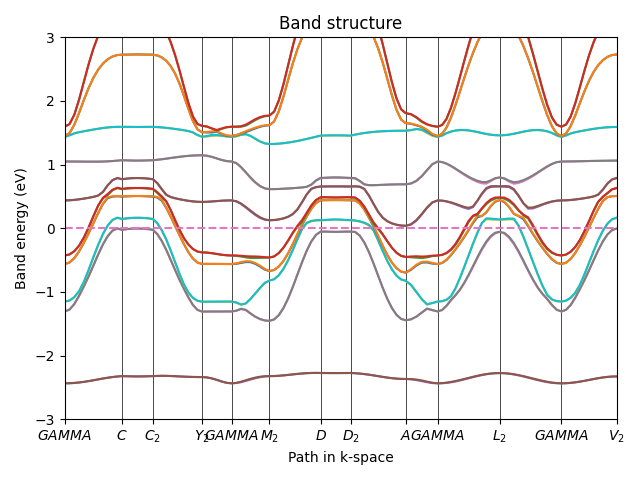
\includegraphics[width=\linewidth]{figures/lieb-nbcl2f-band.png}
        \caption{NbCl$_2$F substitution child, $W=1.454$\,eV.}
    \end{subfigure}
    \caption{\textbf{Candidate-specific SOC learned-Hamiltonian band artifacts from the Lieb-lattice campaign.}
    The panels are native archived outputs, not illustrative reconstructions.  The screen resolves bandwidth and band-crossing diagnostics for each exact structure.  Orbital projection, contributor-site Lieb connectivity, charge distribution, and model calibration remain separate validation targets.}
    \label{fig:lieb-bands}
\end{figure}

Figure~\ref{fig:lieb-bands} shows representative native band artifacts.  The NbOCl$_2$$\rightarrow$NbCl$_2$F example illustrates why explicit structure realization matters: replacing the complete O-equivalent class creates the $x=1$ end member, and the computed band is correspondingly attached to NbCl$_2$F rather than to an unspecified mixed NbO$_{1-x}$F$_x$Cl$_2$.  Intermediate filling now has a concrete next operation---ordered partial substitution in a supercell or a condition-level doping plan---and a parent observation against which descendants can be compared.

The campaign converts a broad open question into a compact experimental and computational frontier.  Li$_2$Ni$_5$OF$_{11}$ descendants are prioritized for charge analysis, orbital projection, and modifications intended to remove the competing Fermi crossing.  NbCl$_2$O and TaCl$_2$O are prioritized for contributor-sublattice connectivity and calibrated electronic confirmation.  Framework hypotheses retain structure acquisition as their next gate.  In every case, the next step is attached to a structure and to the constraint it is intended to resolve.

\subsection{Cross-case system evaluation}
\label{sec:evaluation}

The three studies test whether the same architecture can preserve scientific objects across qualitatively different workflows.  Table~\ref{tab:crosscase} summarizes the observed artifact coverage.  Case I emphasizes source bands, structural transformation, and parent--child provenance.  Case II emphasizes route diversity and a shared verification matrix.  Case III combines all three discovery routes with explicit model execution and iterative structure lineage.

\begin{table}[t]
    \centering
    \caption{\textbf{Cross-case artifact coverage.}}
    \label{tab:crosscase}
    \small
    \setlength{\tabcolsep}{3.5pt}
    \renewcommand{\arraystretch}{1.13}
    \begin{tabularx}{\linewidth}{>{\raggedright\arraybackslash}p{0.20\linewidth}>{\raggedright\arraybackslash}p{0.20\linewidth}XX}
        \toprule
        \textbf{Case} & \textbf{Route and plan coverage} & \textbf{Scientific artifacts} & \textbf{Portfolio output} \\
        \midrule
        2D TM flat band & 1 route; 4 compiled child plans & 3 source bands and 4 child CIFs & Three structure-screening children and one revision route \\
        vdW FM topology & 6 route-bound structure or interface plans & Six candidate verification matrices & Route-diverse portfolio with five shared observables \\
        Fractional-valence Lieb lattice & 3 routes; 7 operator executions; 6 unique children & 17 learned-Hamiltonian band runs & Ranked structure frontier and observable-specific next tasks \\
        \bottomrule
    \end{tabularx}
\end{table}

We use five object-level criteria.  \emph{Constraint coverage} is the fraction of compiled constraints represented in the candidate matrix, including UNKNOWN entries.  \emph{Provenance completeness} requires each populated observation to resolve to a source or execution artifact.  \emph{Structure-backed hypothesis rate} measures which chemical modifications bind to a parent and an executable plan or condition realization.  \emph{Model-route executability} measures whether an approved task has all required input and capability bindings.  \emph{Research continuity} measures whether outputs from one cycle can be consumed without re-entering candidate identity, structure, or evidence manually.  The archived campaigns achieve complete schema coverage and artifact linkage by construction; the case-specific counts in Table~\ref{tab:crosscase} describe how much scientific work was instantiated beyond that contract.

\subsection{Layered comparison and expert benchmark protocol}
\label{sec:benchmark}

To separate the contributions of the language model, \hermes, and the materials service, we define a paired layered benchmark with five arms: base model only; base model with the \hermes research harness; \hermes with retrieval and federated evidence; \hermes plus evidence and \mattransform; and the complete system with \matdag and \matevolve.  Cases are grouped by structure family before assignment so that near-duplicate derivatives do not enter opposite arms.  Each arm receives the same scientific prompt, time budget, accessible public evidence, and output template.

The primary evaluation unit is the candidate-level deliverable, scored on scientific constraint fidelity, source correctness, candidate identity, structural executability, validation specificity, and expert usefulness.  Runtime, tool calls, recovered artifacts, and coverage of decisive observables are recorded as secondary measures.  Expert scoring is performed independently on blinded reports, followed by adjudication of disagreements and a bootstrap confidence interval over source-family groups.

The pre-case calibration contained 12 candidate cases.  After structure-family deduplication and target-class eligibility screening, five independent cases remained for rubric calibration, producing 36 item-level disagreements for adjudication.  This calibration established the scoring manual and blinding workflow.  The report does not convert those calibration judgements into a comparative performance claim; the paired scientific benchmark is reported only when the frozen eligible pool and compute budget support the planned analysis.  The current manuscript therefore grounds its system claims in the end-to-end artifacts above and treats the layered benchmark as the registered evaluation protocol for the next release.

\subsection{Component analysis}

The case studies make the expected contribution of each module observable.  Removing \matspec collapses compound goals into loosely phrased search terms and eliminates a common denominator across routes.  Removing \matevidence loses candidate-linked provenance and conflates direct observations with inference.  Removing \mattransform preserves suggestions but removes child CIFs and parent--child comparison.  Removing \matdag produces structures without capability-checked observables.  Removing \matevolve prevents subsequent cycles from acting on the structures and unresolved constraints already produced.  Removing \hermes leaves the domain service callable, but loses the natural-language research interaction, Profile/Skill policy, controlled continuation, and workflow-level evolution that make the platform usable as a persistent agent.

These are structural ablations of the artifact graph, not substitutions of one model score for another.  They define the rows of the paired benchmark and explain why the complete platform is evaluated on scientific deliverables rather than response fluency alone.
